% Taylor & Francis LaTeX template for authors (Interact layout + APA reference style)
% source: https://www.overleaf.com/latex/templates/taylor-and-francis-latex-template-for-authors-interact-layout-plus-apa-reference-style/jqhskrsqqzfz

\documentclass[]{./cls/interact}

% Template Preamble

\usepackage{epstopdf}				% To incorporate .eps illustrations using PDFLaTeX, etc.
\usepackage[caption=false]{subfig}		% Support for small, `sub' figures and tables
%\usepackage[nolists,tablesfirst]{endfloat}	% To `separate' figures and tables from text if required
%\usepackage[doublespacing]{setspace}		% To produce a `double spaced' document if required
%	\setlength\parindent{24pt}		% To increase paragraph indentation when line spacing is doubled

% Citation support using apacite.sty. 
\usepackage[natbibapa,nodoi]{apacite}					% Citation support using apacite.sty. 
\setlength\bibhang{12pt}						% To set the indentation in the list of references using apacite.sty. 
\renewcommand\bibliographytypesize{\fontsize{10}{12}\selectfont}	% To set the list of references in 10 point font using apacite.sty. 

% Theorem-like structures provided by amsthm.sty
\theoremstyle{plain}				
\newtheorem{theorem}{Theorem}[section]
\newtheorem{lemma}[theorem]{Lemma}
\newtheorem{corollary}[theorem]{Corollary}
\newtheorem{proposition}[theorem]{Proposition}

\theoremstyle{definition}
\newtheorem{definition}[theorem]{Definition}
\newtheorem{example}[theorem]{Example}

\theoremstyle{remark}
\newtheorem{remark}{Remark}
\newtheorem{notation}{Notation}

% Custom Preamble

% Important packages
\usepackage{hyperref}	% automatic pdf outline and citations hyperlinks
\usepackage{placeins} 	% for FloatBarrier

% Paths
\newcommand{\pathBIB}{./bib}
\newcommand{\pathFIG}{./figures}
% Paths for work in progress versions
%\newcommand{\pathFIG}{../output/graphs} 	% pools from my R output folder
%\newcommand{\pathBIB}{../../statsLib}		% pools from my bibliography

% Macros
\newcommand{\norm}[1]{\left\lVert#1\right\rVert} % for l2 norm in equations

% Begin Manuscript
\begin{document}

\articletype{SUPPLEMENTARY MATERIAL}	% Specify the article type or omit as appropriate

% Manuscript details
\title{High Dimensional Imputation for the Social Sciences: A Comparison of State-of-the-Art Methods}

\author{
\name{
	Edoardo Costantini\textsuperscript{a} \thanks{CONTACT Edoardo Costantini. Email: e.costantini@tilburguniversity.edu},
	Kyle M. Lang\textsuperscript{a},
	Tim Reeskens\textsuperscript{b}, and
	Klaas Sijtsma\textsuperscript{a}
	}
\affil{
	\textsuperscript{a}Tilburg University, Department of Methodology and Statistics;
	\textsuperscript{b}Tilburg University, Department of Sociology
	}
}

\maketitle

% Body
\section{Software and other computational details}

The code to run the simulation was written in the R statistical programming language (version 4.0.3). 
All experiments were run using a 2.6 GHz Intel Xeon(R) Gold 6126 processor, 523.78 GB of Memory. The
operating system was Windows Server 2012 R2.
Computations were run in parallel across 30 cores. 
Parallel computing was implemented using the R package \emph{parallel} and to ensure replicability 
of the findings seeds were set using the method by \cite{lecuyer:2002} implemented in the R package 
\emph{rlecuyer}.
Code to run the studies can be found at \url{https://github.com/EdoardoCostantini/imputeHD-comp}.
In the following, each step of the simulation procedure is described in details for both experiments.

\section{Convergence check details}

	Convergence of the imputation models was assessed in a preprocessing step.
	Before running the actual simulation studies, 10 datasets were generated according to each experimental set up.
	Missing values in each dataset were imputed by running 5 parallel imputation chains for each Multiple Imputation 
	method.
	Convergence was checked by plotting the mean of the imputed values for each variable in each stream, against the 
	iteration number.
	In each parallel run, all the MI algorithms run for 250 iterations.
	The imputation algorithms were considered to have converged after 50 iterations, after which 10 imputed data 
	sets were store and used for the subsequent standard complete-data analysis and pooling.
	The only exception was blasso, which required approximately 2000 iterations for convergence.

\section{Ridge penalty cross-validation details}
	The ridge penalty used in the bridge algorithm was fixed across iterations .
	The value used in the simulation was determined by means of cross-validation in a pre-processing phase.
	The grid of possible values for the ridge penalty was $10^{-1}, 10^{-2}, ..., 10^{-8}$.
	For each of 100 data repetitions, bridge imputation was performed with each of the different penalty parameters
	and used to obtain 10 differently imputed datasets.
	For each data replication, the Fraction of Missing Information (FMI) \citep{savaleiRhemtulla:2012} associated with 
	each parameter in the analysis models of interest (see next section for details) was computed and then averaged across 
	repetitions.
	The mean of these average parameter FMIs was used as a composite measure of FMI associated with each ridge penalty
	value.
	Finally, the penalty value with the smallest composite FMI was selected.

\section{Additional Figures}

\subsubsection{Experiment 1}

	Figures \ref{fig:exp1bias} and \ref{fig:exp1cir} report the Percentage Relative Bias and Confidence Interval 
	Coverage, respectively, for each parameter estimate in the saturated model described above. 
	In the figures, single horizontal lines, representing the PRB (or CIC) of a parameter estimate for a single 
	variable, combine to form larger horizontal bars giving an aggregate account of how each method performed 
	across multiple variables with missing values.

	\paragraph{Means} 
	Focusing first on the item means (top rows), all methods achieved a bias that is smaller than the 10\% threshold 
	for all item means, in all conditions.
	The largest PRB is within 10 percentage points from 0 for all methods.
	Looking at relative performances, in all conditions, MI-OP provided negligible bias, and IURR and MI-PCA resulted 
	in the smallest estimation bias among the other methods.
	
	In the conditions with low proportion of missing values (condition 1 and 2), only the tree-based MI methods,
	missForest, and CC showed CIC significantly different from nominal coverage rates.
	In the conditions with high proportion of missing values (condition 3 and 4), all methods showed some signs 
	of either under-coverage or over-coverage of the true values, with CICs outside of the interval $(.94, .96)$.
	The only exceptions to the trend were MI-OP, MI-PCA, and Bridge which showed non-significant deviations from 
	nominal coverage for almost all estimates.

	\paragraph{Variances} 
	Moving to the item variances (central rows), IURR, blasso, and the tree-based methods resulted in the lowest
	biases across all conditions, even in the high-dim-high-pm condition (condition 4).
	These low biases were mostly paired with low deviations from nominal coverage, except for the high-dim-high-pm
	condition (condition 4) where IURR and the tree-based methods resulted in extreme under-coverage of the true item 
	variances ($CIC << .9$).
	Apart from MI-OP, Blasso was the method with best coverage in this final condition.
	
	Directly using regularized regression within the imputation models (DURR) showed poor performance with regard 
	to the item variances: in all conditions but the first, it led to large (negative) bias, with a PRB as large as 10\% in 
	the last condition, accompanied by clear signs of CI under-coverage.
	Bridge was the only MI method showing larger bias than DURR, in all the high-dimensional conditions (2 and 4):
	imputing the data with Bridge led to all item variance estimates showing a bias larger than 20\% the size of the
	true value.

	MI-PCA also showed poor performance with a noticeable positive bias in all conditions that became extreme in
	high-dim-high-pm condition (condition 4), where the PRBs exceeded 20\%.
	This poor performance was reflected in extreme confidence interval under-coverage of the true item variances in
	the final experimental condition.

	Single data imputation with missForest and complete case analysis led to substantial negative bias and 
	CI under-coverage for all item variances, even in condition 1.

	\paragraph{Covariances}
	Finally, the third row in Figure \ref{fig:exp1bias} shows the estimation bias for the 15 covariances between 
	the 6 items with missing values.
	As covariances depend on two variables, recovering the correct estimates after imputation is 
	more difficult than with means and variances.
	This explains the generally worse performance reported in the figure.

	Indirect Use of Regularized Regression (IURR) performed noticeably better than most other methods, 
	with negligible negative bias and acceptable coverage for all covariances in conditions 1, 2 and 3, 
	but it struggled with a large negative bias and extreme under-coverage for the majority of the 15 
	covariances in the high-dim-high-pm condition (condition 4).
	
	MI-PCA showed negligible negative bias of the covariance estimates in all conditions, performing as 
	well as MI-OP in all but the last condition, where it still maintained acceptably low values of PRB 
	($|PRB| < 10\%$).
	Furthermore, MI-PCA showed virtually no deviation from nominal coverage, with a CIC pattern similar to 
	that of MI-OP, in all but the last condition, where it manifested only mild \emph{over}-coverage of the 
	items covariances.

	All other methods, including DURR, showed absolute PRBs larger than the 10\% threshold in all but the 
	first condition, with mild to extreme signs of under-coverage.
	Bridge displayed acceptably low biases and coverage in the low dimensional conditions, and 
	extremely large biases and low CI coverage in all the high dimensional conditions.
	Single data approaches, like missForest and CC, showed extreme bias and under-coverage of covariances between 
	items with missing values, even in condition 1.

\begin{figure}
\centering
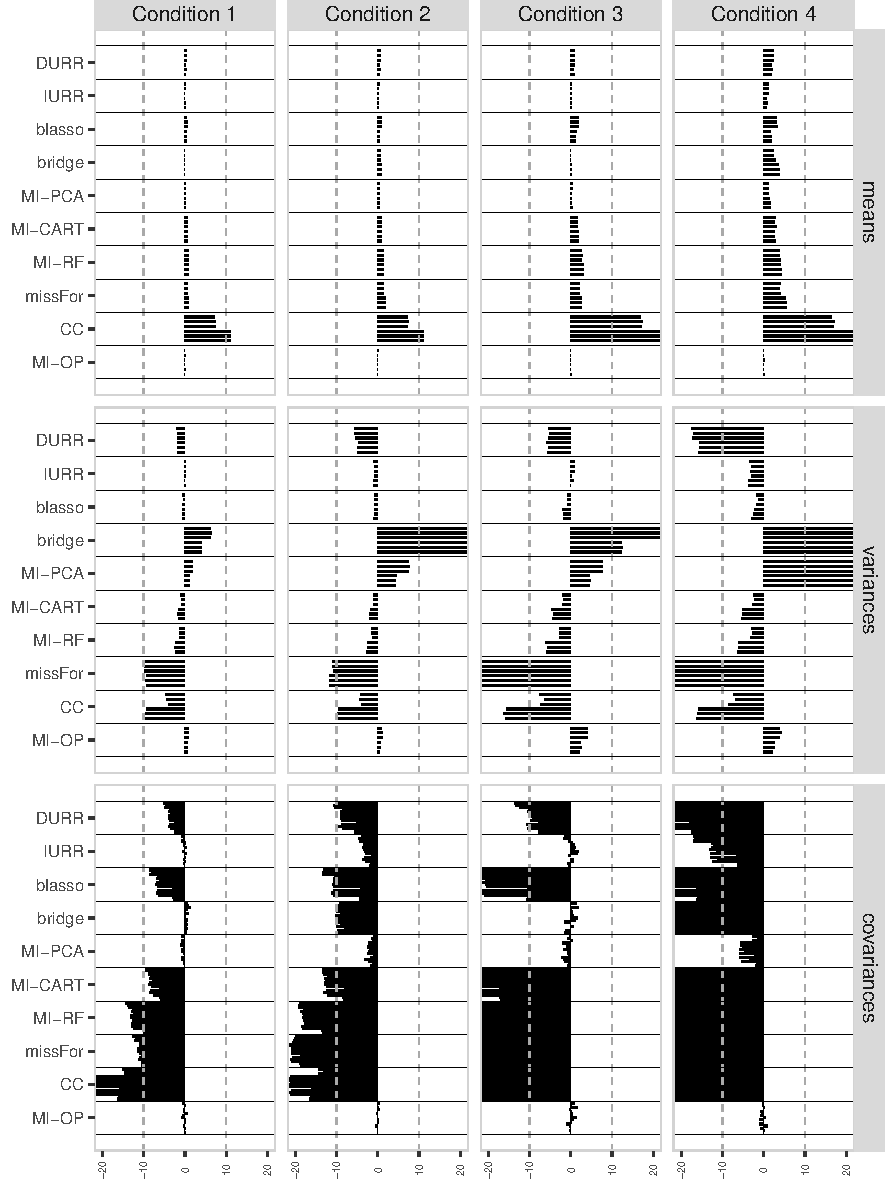
\includegraphics{\pathFIG/exp1_bias.pdf}
\caption{\label{fig:exp1bias}
	Percent Relative Bias (PRB) for item means, variances, and covariances.
	For every method, single horizontal lines, representing the PRB of a parameter estimate on 
	a single variable (or pair of variables), combine to form larger horizontal bars giving an 
	aggregate account of how each method performed across multiple variables with missing values.
	}
\end{figure}

\begin{figure}
\centering
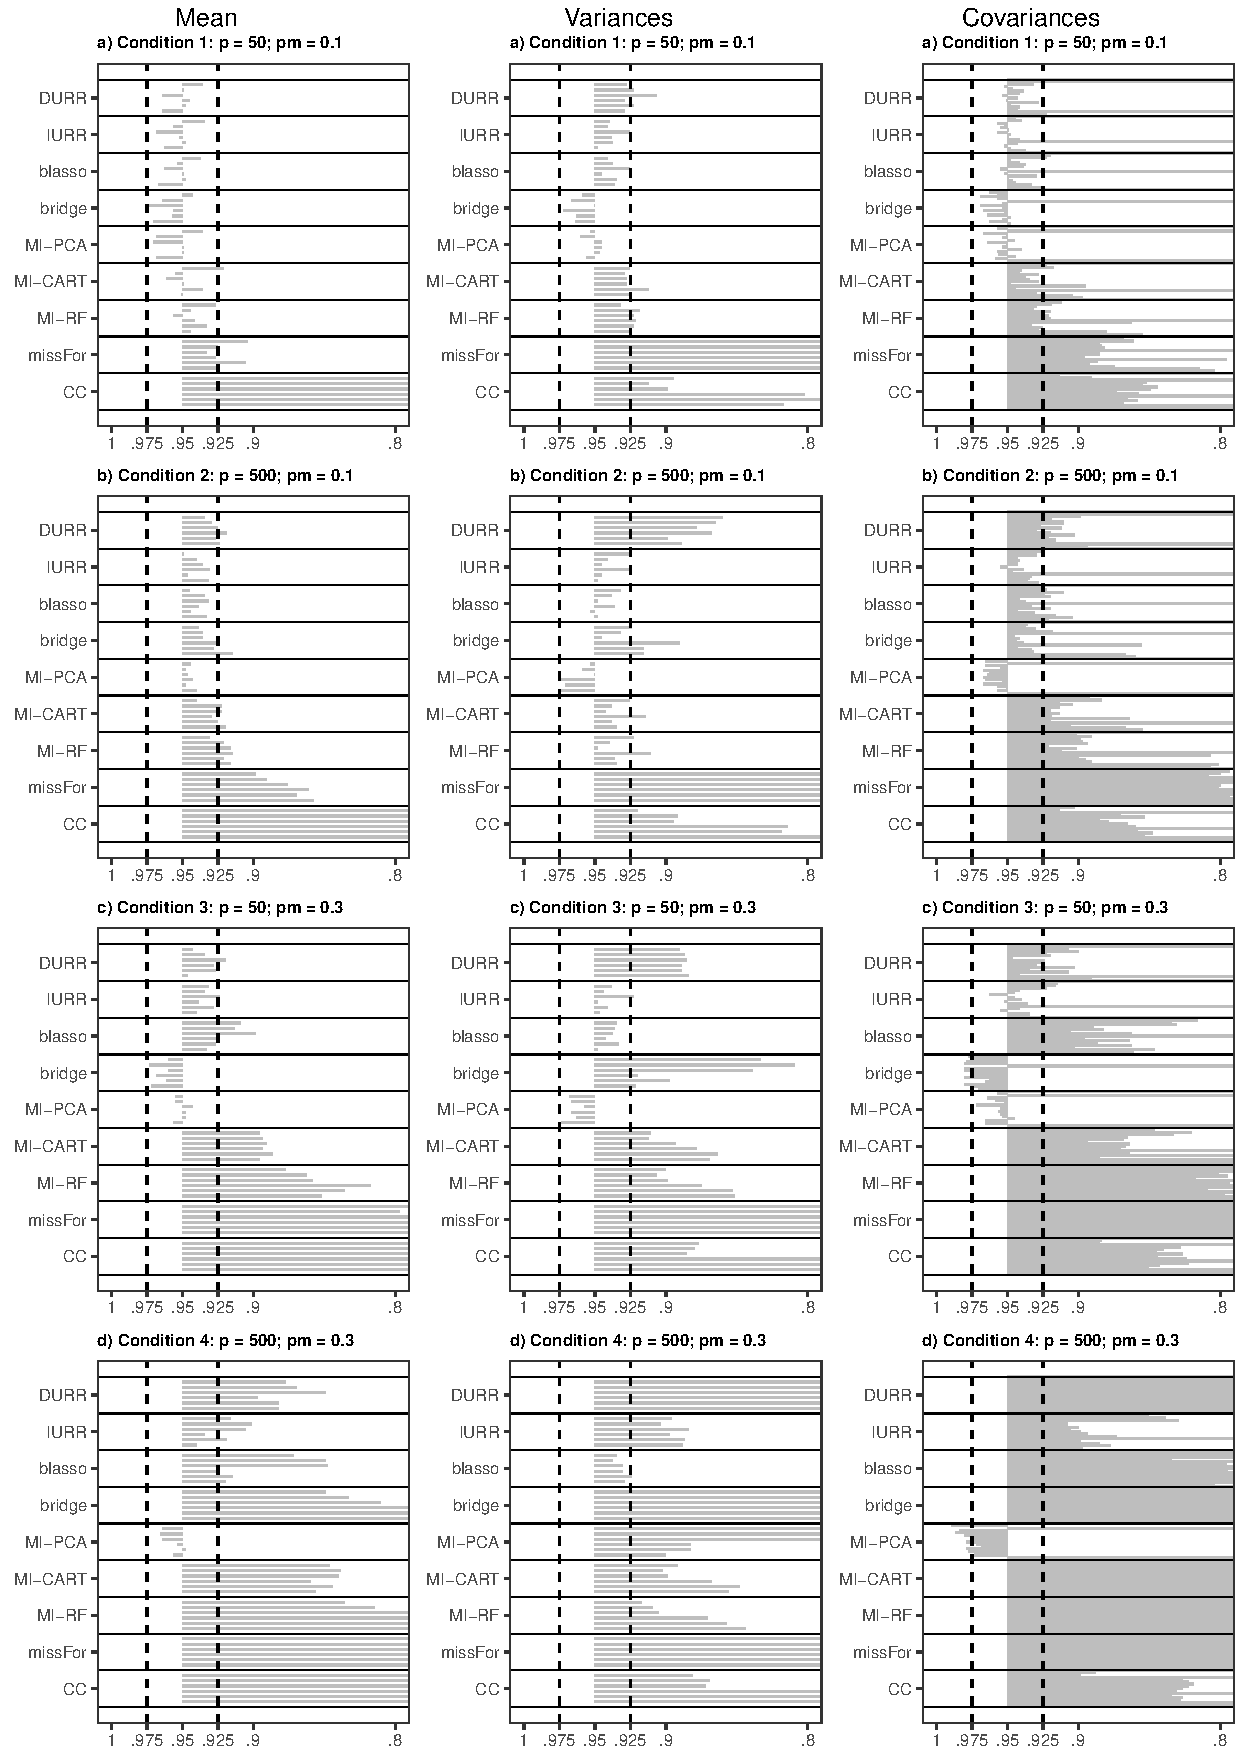
\includegraphics{\pathFIG/exp1_CI.pdf}
\caption{\label{fig:exp1cir}
	Confidence Interval Coverage (CIC) for item means, variances, and covariances. 
	For every method, single horizontal lines, representing the CIC of a parameter estimate on 
	a single variable (or pair of variables), combine to form larger horizontal bars giving an 
	aggregate account of how each method performed across multiple variables with missing values.
	}
\end{figure}

\FloatBarrier

%% EXP 2

\subsubsection{Experiment 2}

	Figures \ref{fig:exp2bias} and \ref{fig:exp2cir} report the PRB and CIC of the estimated means, variances, 
	and covariances of the 10 items with missing values in the first four conditions of Experiment 2, 
	the ones characterized by high factor loadings (strong latent structure).
	Figures \ref{fig:exp2bias58} and \ref{fig:exp2cir58} in appendix reports the same values for the low 
	factor loading conditions.

	\paragraph{Means}
	All methods provided unbiased estimates of the item means with PRBs that were almost 0 for all items.
	As the proportion of missing cases increased (conditions 3 and 4) there was a slight increase in 
	PRB values for all methods except IURR, bridge, and MI-PCA. 
	However, only Complete Case analysis led to unacceptable bias in these scenarios.
	DURR, IURR and MI-PCA also showed little to no deviations from nominal coverage in all conditions, 
	while blasso, MI-CART, MI-RF, and bridge led to significant under-coverage when the proportion of 
	missing cases was high (conditions 3 and 4). 
	missForest also led to extreme under-coverage of the true values.
	
	\paragraph{Variances}
	All MI methods, except Bridge, resulted in acceptable bias levels for item variances estimates in all conditions, 
	but the least biased estimates were obtained by MI-OP, IURR and MI-PCA.
	CIC decreased as the proportion of missing cases increased (from condition 1 and 2 to conditions 3 and 4).
	For high $pm$, only IURR and MI-PCA maintained CICs mostly within the range .94-.96, while blasso and the MI tree-based 
	methods led to mild to extreme under-coverage (CIC < 90\%).

	The large positive bias (and low CIC) for the item variances that afflicted MI-PCA in the multivariate-normal set up 
	(figures \ref{fig:exp1bias} and \ref{fig:exp1cir}) is not present in figures \ref{fig:exp2bias} and \ref{fig:exp2cir}.
	However, that pattern reappeared when the latent structure was weak, as can be seen in Figure \ref{fig:exp2bias58} 
	and \ref{fig:exp2cir58} in the Appendix (conditions 5 to 8, factor loadings between .5 and .8).
	Single data approaches, missForest and CC, showed again extreme (negative) bias and CI under-coverage in 
	almost all conditions.

	\paragraph{Covariances}
	For all the conditions with high factor loadings in experiment 2, IURR and DURR showed acceptable covariance biases 
	($|\text{PRB}|<10\%$).
	However, they led to large negative bias in all the conditions with low factor loadings (see \ref{fig:exp2bias58} and 
	\ref{fig:exp2cir58} in the Appendix)
	The other methods followed the same pattern as in experiment 1: the MI-PCA approach resulted in the lowest 
	bias and deviation from nominal coverage for the covariances of the observed items; 
	all other methods led to large negative biases and mild-to-extreme under-coverage for all the covariances, 
	in all conditions.

	\paragraph{Factor Loadings}
	Figure \ref{fig:exp2fl14} shows the PRB values for all the factor loadings estimated by
	the Confirmatory Factor Analysis described above. 
	Most MI-Methods provided acceptably low bias for these estimates in all conditions except the one with 
	both large proportion of missing values and high dimensional input data matrix (condition 4 and 8).

	MI-OP, IURR, and MI-PCA outperformed all other methods and produced virtually unbiased estimates
	of the factor loadings in all conditions.
	In particular, MI-PCA outperformed IURR when factor loadings were low (panel b, conditions 5 to 8), 
	maintaining inconsequential biases even when data were high-dimensional and the proportion of missing 
	values was high.

%\begin{rotatepage}	
\begin{figure}
	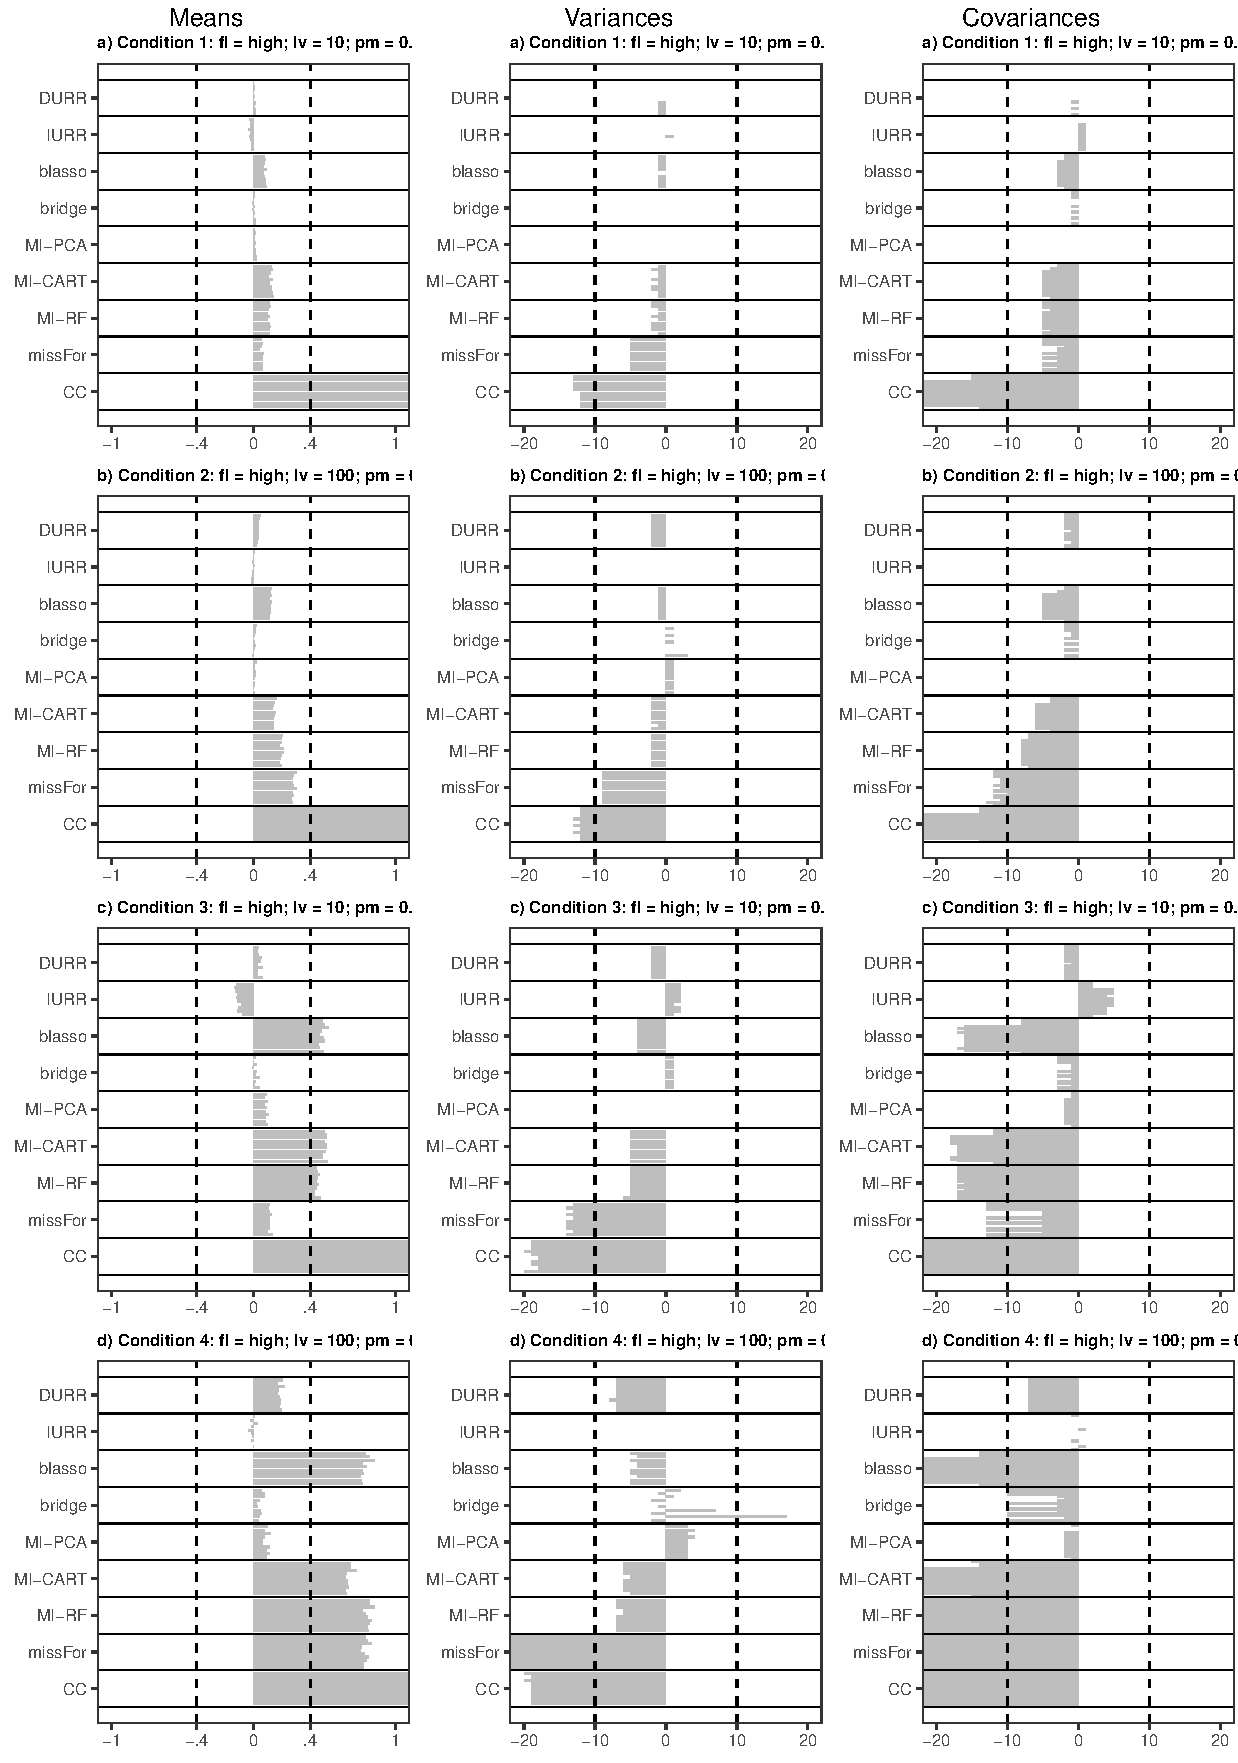
\includegraphics{\pathFIG/exp2_semR_bias_14.pdf}
\caption{PRBs for the means, variances and covariances (PRB) for condition 1 to 4.
	For every method, single horizontal lines, representing the PRB of a parameter estimate on 
	a single variable (or pair of variables), combine to form larger horizontal bars giving an 
	aggregate account of how each method performed across multiple variables with missing values.
}
\label{fig:exp2bias14}
\end{figure}

\begin{figure}
	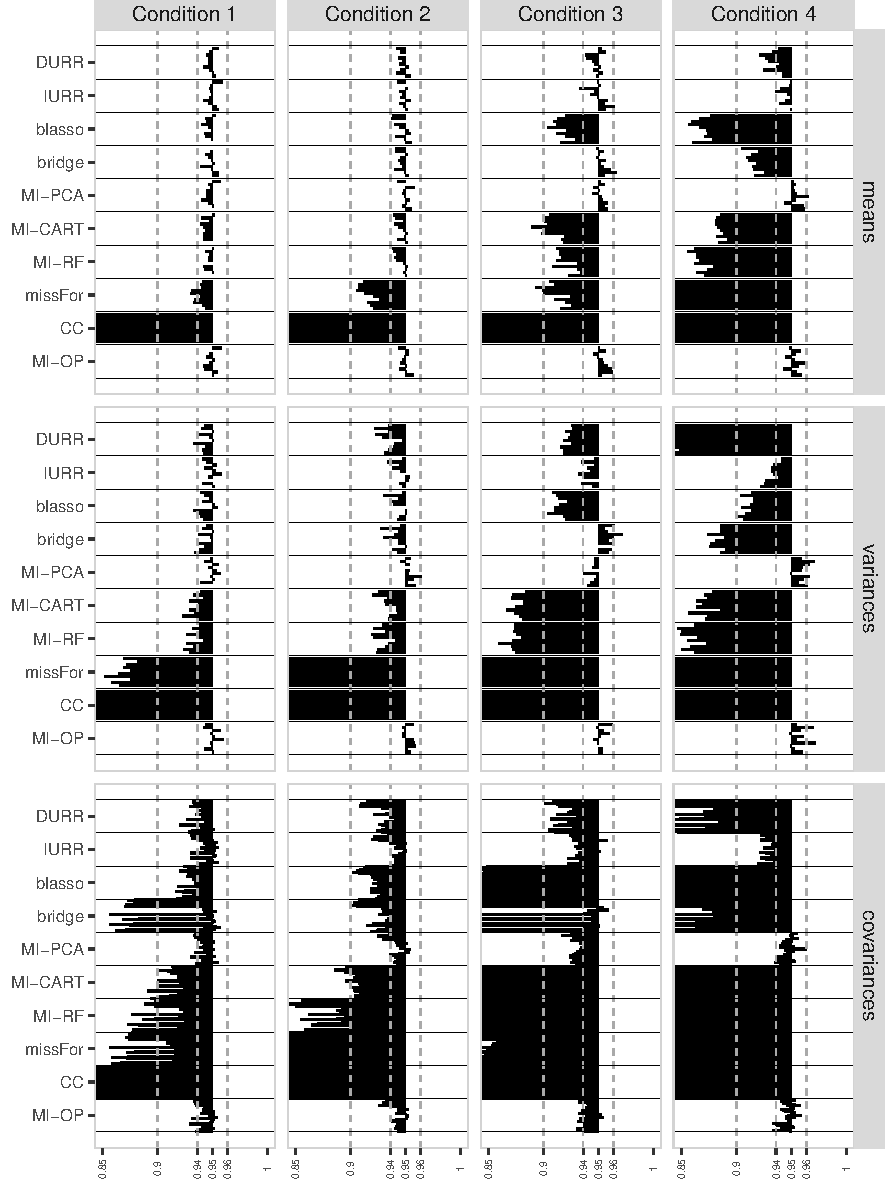
\includegraphics{\pathFIG/exp2_semR_ci_14.pdf}
\caption{CIC for the means, variances, and covariances for condition 1 to 4.
	For every method, single horizontal lines, representing the CIC of a parameter estimate on 
	a single variable (or pair of variables), combine to form larger horizontal bars giving an 
	aggregate account of how each method performed across multiple variables with missing values.
}
\label{fig:exp2cir14}
\end{figure}


\begin{figure}
	\centering
	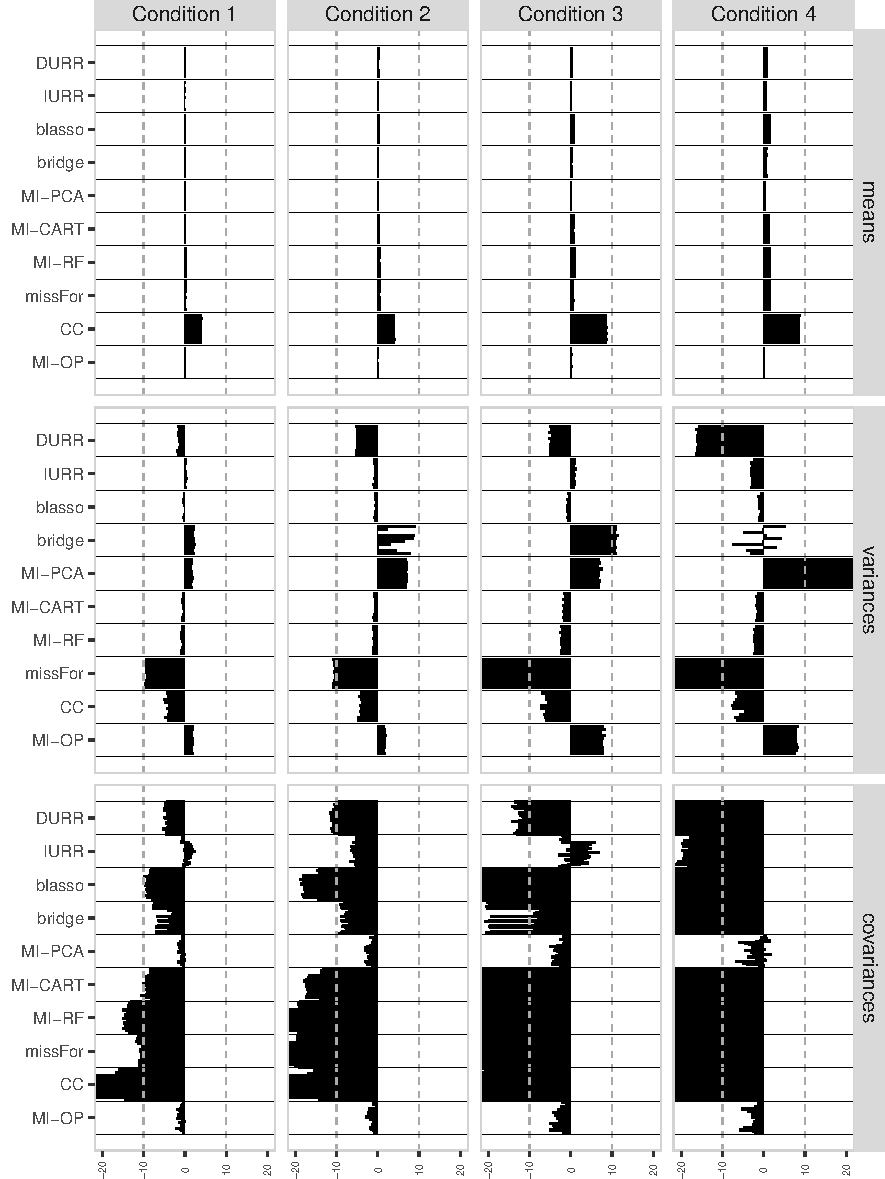
\includegraphics{\pathFIG/exp2_semR_bias_58.pdf}
	\caption{Bias estimation for the means (SB), variances and covariances (PRB) for condition 5 
			to 8.}
	\label{fig:exp2bias58}
\end{figure}

\begin{figure}
	\centering
	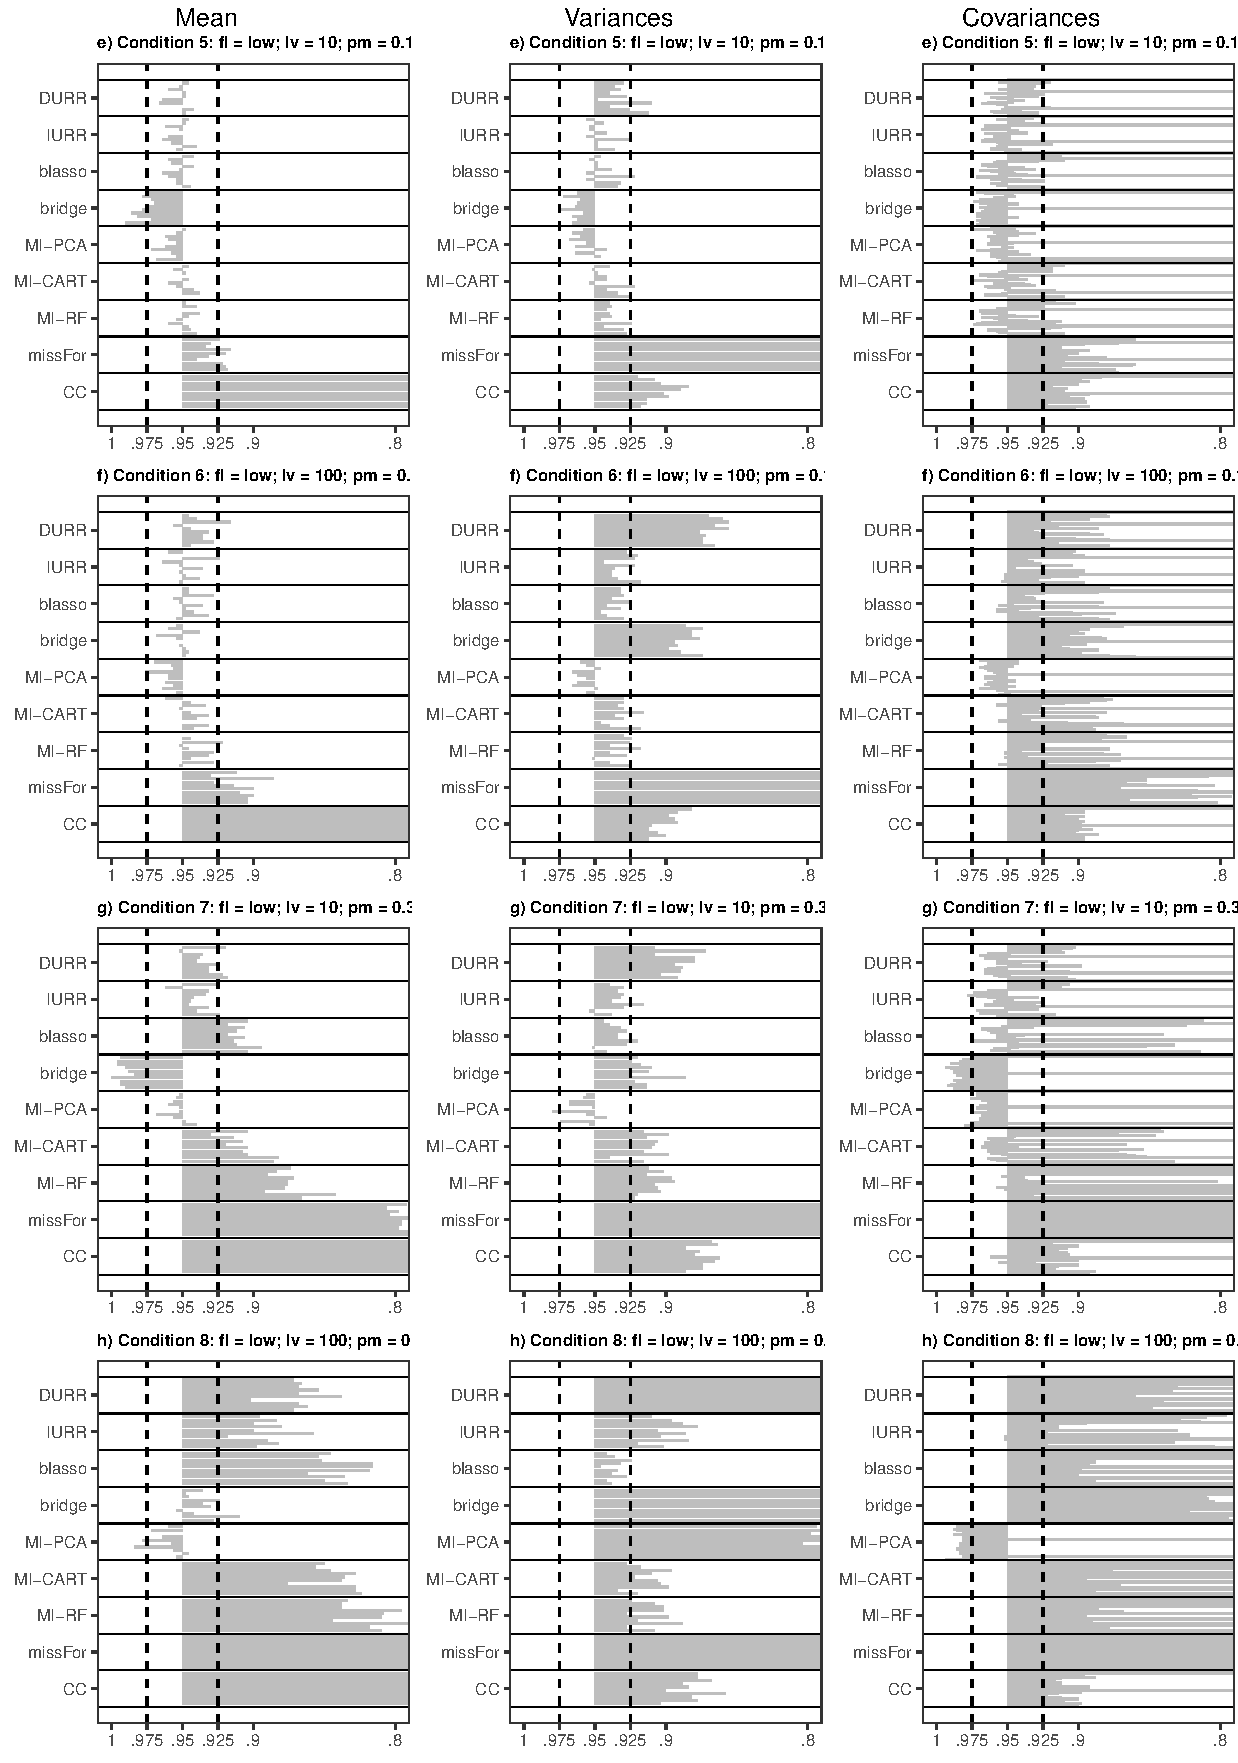
\includegraphics{\pathFIG/exp2_semR_ci_58.pdf}
	\caption{Confidence Interval Coverage (CIC) for the means, variances, and covariances 
			for condition 5 to 8.}
	\label{fig:exp2cir58}
\end{figure}

\begin{figure}
	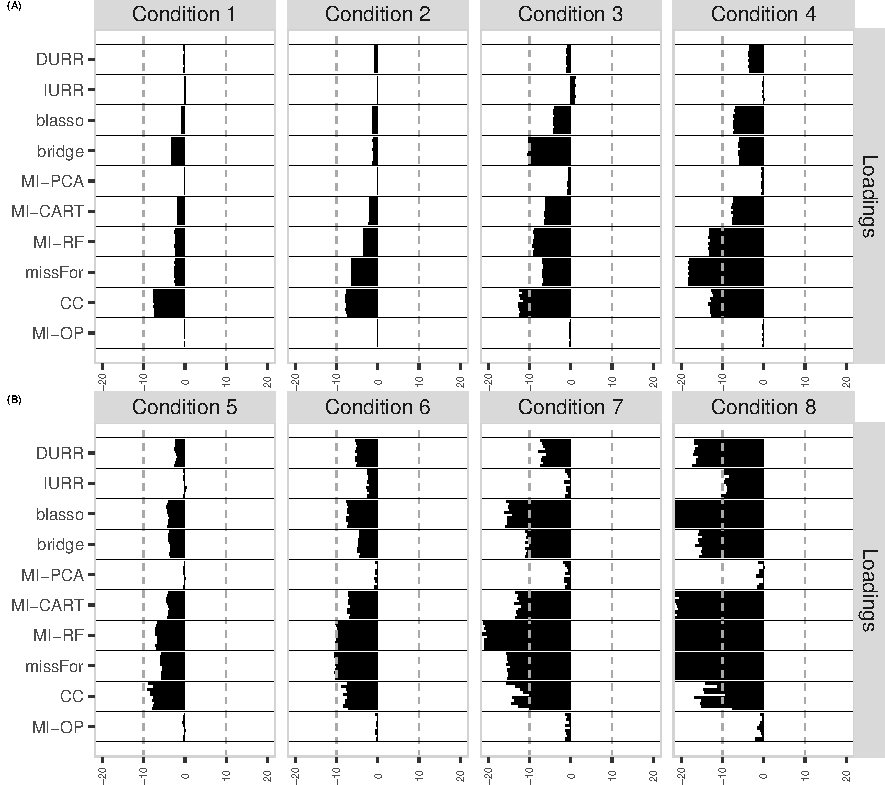
\includegraphics{\pathFIG/exp2_CFA_lambda_BPR.pdf}
	\caption{
		Percent Relative Bias (PRB) for the factor loadings in conditions 1 to 4 (panel A) 
		and conditions 5 to 8 (panel B).
		Within each panel, for every method, single horizontal lines report the PRB of the 
		factor loading estimation for each item with missing values.
		}
\label{fig:exp2fl14}
\end{figure}

\begin{figure}
	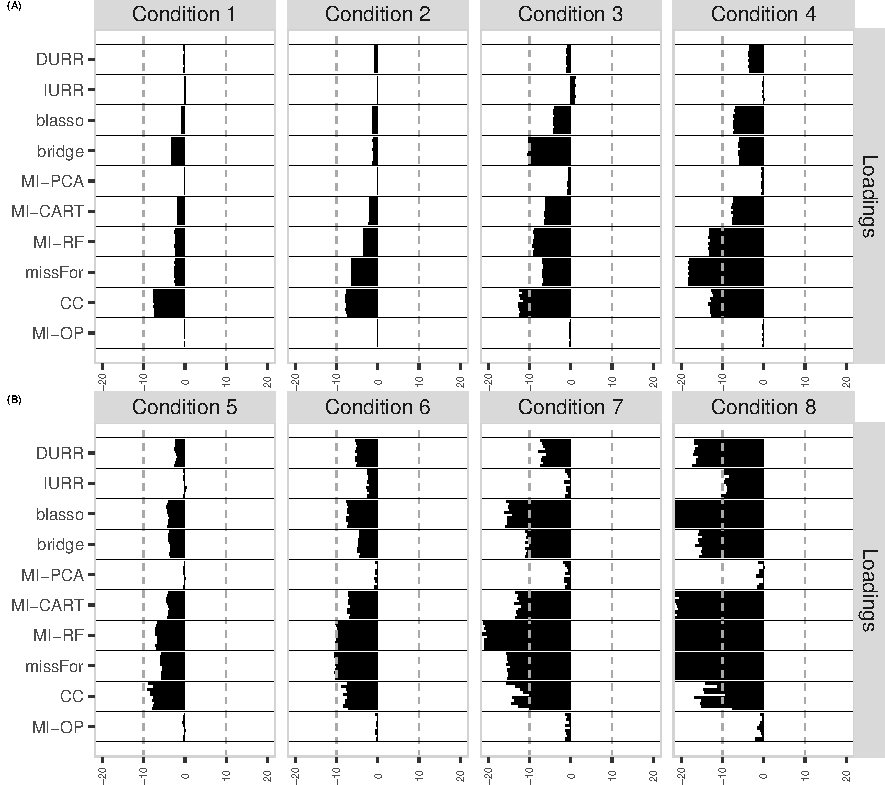
\includegraphics{\pathFIG/exp2_CFA_lambda_BPR.pdf}
	\caption{
		Percent Relative Bias (PRB) for the factor loadings in conditions 1 to 4 (panel A) 
		and conditions 5 to 8 (panel B).
		Within each panel, for every method, single horizontal lines report the PRB of the 
		factor loading estimation for each item with missing values.
		}
\label{fig:exp2fl14}
\end{figure}

\FloatBarrier

\subsubsection{Resampling Study}

Supplements to resampling study

\begin{figure}
	\centering
	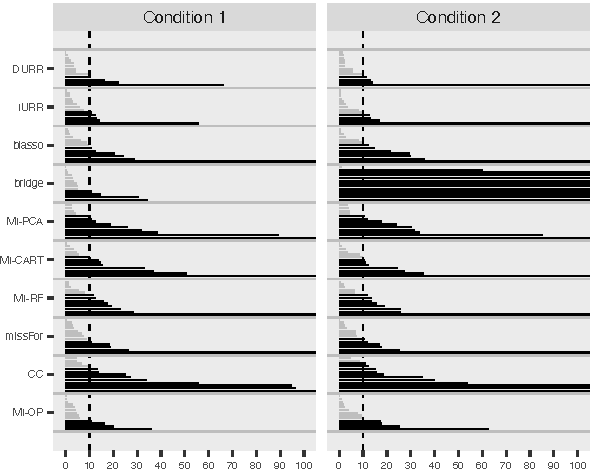
\includegraphics{\pathFIG/exp4_imp_bias_allParms_m1.pdf}
	\caption{PRBs for all the model parameters in model 1. 
		The order of the bars is based on the absolute value of the PRBs.
		The values for the intercept, the focal regression coefficient, and the regression coefficient with which most 
		methods struggle (Largest Bias) are highlighted}
	\label{fig:exp4bias_m1}
\end{figure}

\begin{figure}
	\centering
	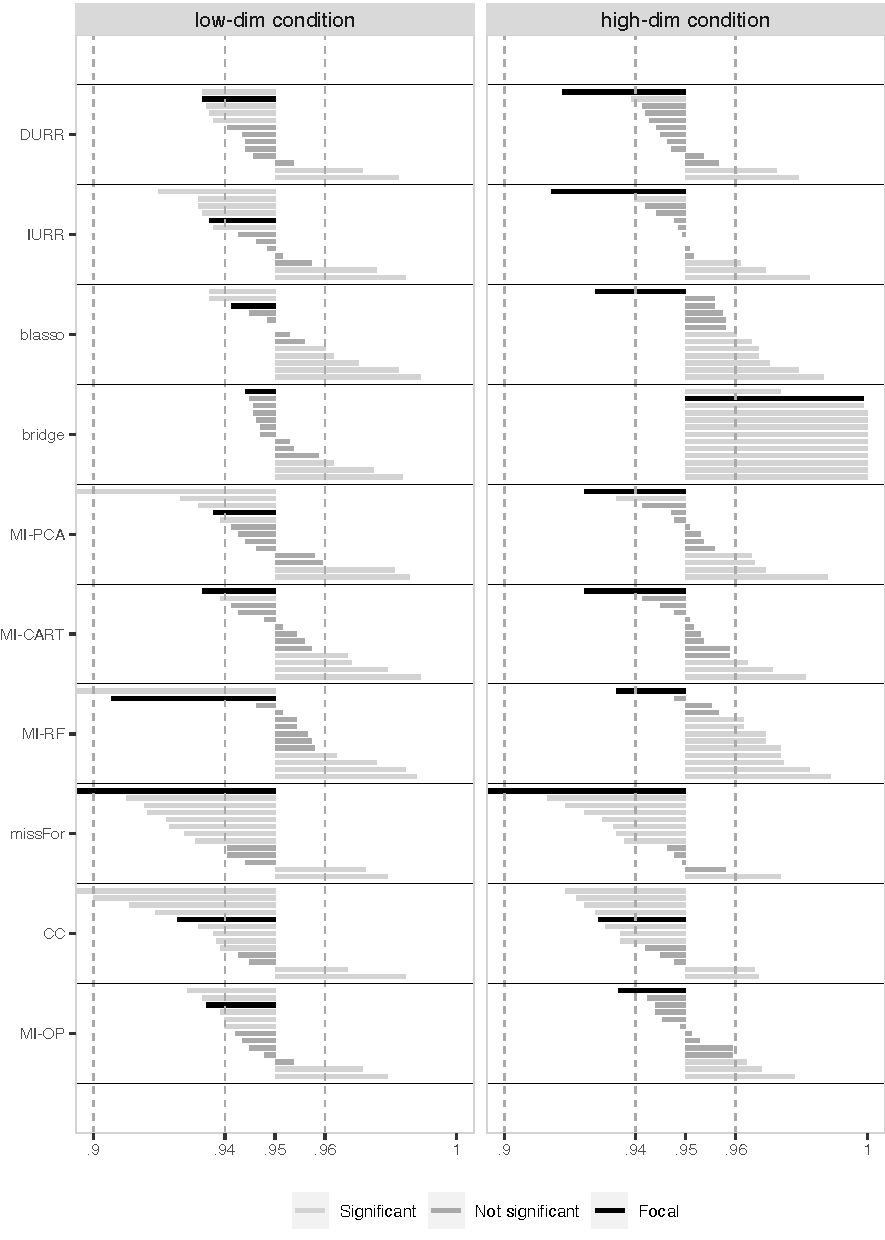
\includegraphics{\pathFIG/exp4_imp_ci_allParms_m1.pdf}
	\caption{CIC for all model parameter in model 1.
		Bars are sorted in by ascending value.
		The values for the intercept, the focal regression coefficient, and the regression coefficient with which most 
		methods struggle (Largest Bias) are highlighted}
	\label{fig:exp4cir_m1}
\end{figure}

\FloatBarrier

\subsection{Experiment 3: Resampling study}

	Figure \ref{fig:exp4_bias_allP} reports the absolute values of the PRBs for every parameter in Model 2, 
	ordered by size, under each of the different imputation methods.

	comment here

	Figure \ref{fig:exp4_ci_allP} reports the CIC for each parameter estimate in model 2.
	When using MI-OP, CICs showed a deviation from nominal coverage for only two parameters, with a slight 
	tendency toward over-coverage.

	comment here

	the important thing is that last comment about the 

	All MI methods led to significant under-coverage of the true parameter values with CIC smaller than the 
	threshold value 0.94.
	Although coverage of the true values was not particularly good for any of the methods selected, the Gold Standard
	confidence intervals were also under-covering the true value of $\beta_{1}$ in Model 1.
	This was likely due to the right-skewed nature of the distribution of the dependent variable (euthanasia 
	acceptance).
	Most MI imputation methods achieved coverages similar to that of the Gold Standard method, and more importantly 
	their relative difference, compared to the GS coverages, was in line with what can be seen for $\beta_{1}$ in Model 2.

\begin{figure}
	\centering
	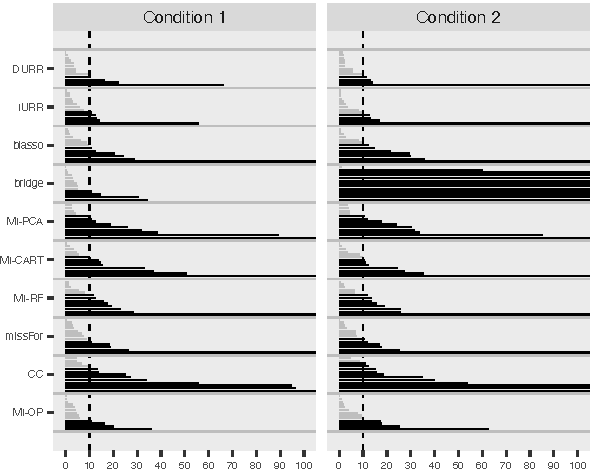
\includegraphics{\pathFIG/exp4_imp_bias_allParms_m1.pdf}
	\caption{PRBs for all the model parameters in model 1. 
		The order of the bars is based on the absolute value of the PRBs.
		The values for the intercept, the focal regression coefficient, and the regression coefficient with which most 
		methods struggle (Largest Bias) are highlighted}
	\label{fig:exp4_bias_allP}
\end{figure}

\begin{figure}
	\centering
	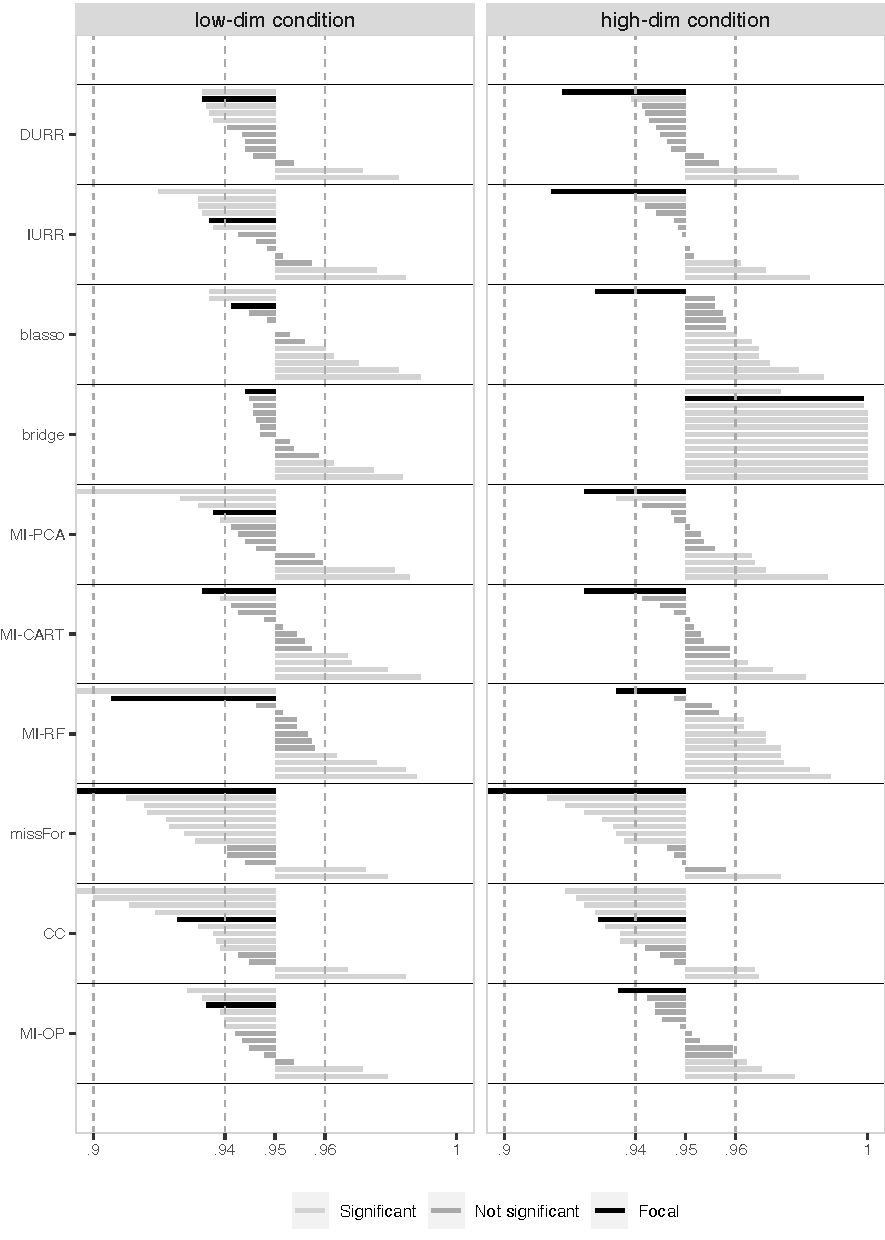
\includegraphics{\pathFIG/exp4_imp_ci_allParms_m1.pdf}
	\caption{CIC for all model parameter in model 1.
		Bars are sorted in by ascending value.
		The values for the intercept, the focal regression coefficient, and the regression coefficient with which most 
		methods struggle (Largest Bias) are highlighted}
	\label{fig:exp4_ci_allP}
\end{figure}

\end{document}
